% This is "sig-alternate.tex" V2.1 April 2013
% This file should be compiled with V2.5 of "sig-alternate.cls" May 2012
%
% This example file demonstrates the use of the 'sig-alternate.cls'
% V2.5 LaTeX2e document class file. It is for those submitting
% articles to ACM Conference Proceedings WHO DO NOT WISH TO
% STRICTLY ADHERE TO THE SIGS (PUBS-BOARD-ENDORSED) STYLE.
% The 'sig-alternate.cls' file will produce a similar-looking,
% albeit, 'tighter' paper resulting in, invariably, fewer pages.
%
% ----------------------------------------------------------------------------------------------------------------
% This .tex file (and associated .cls V2.5) produces:
%       1) The Permission Statement
%       2) The Conference (location) Info information
%       3) The Copyright Line with ACM data
%       4) NO page numbers
%
% as against the acm_proc_article-sp.cls file which
% DOES NOT produce 1) thru' 3) above.
%
% Using 'sig-alternate.cls' you have control, however, from within
% the source .tex file, over both the CopyrightYear
% (defaulted to 200X) and the ACM Copyright Data
% (defaulted to X-XXXXX-XX-X/XX/XX).
% e.g.
% \CopyrightYear{2007} will cause 2007 to appear in the copyright line.
% \crdata{0-12345-67-8/90/12} will cause 0-12345-67-8/90/12 to appear in the copyright line.
%
% ---------------------------------------------------------------------------------------------------------------
% This .tex source is an example which *does* use
% the .bib file (from which the .bbl file % is produced).
% REMEMBER HOWEVER: After having produced the .bbl file,
% and prior to final submission, you *NEED* to 'insert'
% your .bbl file into your source .tex file so as to provide
% ONE 'self-contained' source file.
%
% ================= IF YOU HAVE QUESTIONS =======================
% Questions regarding the SIGS styles, SIGS policies and
% procedures, Conferences etc. should be sent to
% Adrienne Griscti (griscti@acm.org)
%
% Technical questions _only_ to
% Gerald Murray (murray@hq.acm.org)
% ===============================================================
%
% For tracking purposes - this is V2.0 - May 2012

\documentclass{main}
\pagenumbering{arabic}

\usepackage{listings}
\usepackage{caption}

\lstset{
language=C++,
basicstyle=\small\ttfamily,
numbers=left,
numbersep=5pt,
xleftmargin=20pt,
frame=tb,
framexleftmargin=20pt
}

\begin{document}

% Copyright
%\setcopyright{acmcopyright}
%\setcopyright{acmlicensed}
%\setcopyright{rightsretained}
%\setcopyright{usgov}
%\setcopyright{usgovmixed}
%\setcopyright{cagov}
%\setcopyright{cagovmixed}


\title{Associative Reduction in Halide}

%\numberofauthors{3}
%\author{
%% 1st. author
%\alignauthor
%Ben Trovato\titlenote{Dr.~Trovato insisted his name be first.}\\
%       \affaddr{Institute for Clarity in Documentation}\\
%       \affaddr{1932 Wallamaloo Lane}\\
%       \affaddr{Wallamaloo, New Zealand}\\
%       \email{trovato@corporation.com}
%% 2nd. author
%\alignauthor
%G.K.M. Tobin\titlenote{The secretary disavows
%any knowledge of this author's actions.}\\
%       \affaddr{Institute for Clarity in Documentation}\\
%       \affaddr{P.O. Box 1212}\\
%       \affaddr{Dublin, Ohio 43017-6221}\\
%       \email{webmaster@marysville-ohio.com}
%% 3rd. author
%\alignauthor Lars Th{\o}rv{\"a}ld\titlenote{This author is the
%one who did all the really hard work.}\\
%       \affaddr{The Th{\o}rv{\"a}ld Group}\\
%       \affaddr{1 Th{\o}rv{\"a}ld Circle}\\
%       \affaddr{Hekla, Iceland}\\
%       \email{larst@affiliation.org}
%}

\maketitle
\begin{abstract}

<Insert abstracts here>

\end{abstract}


%
%  Use this command to print the description
%
\printccsdesc

%\keywords{ACM proceedings; \LaTeX; text tagging}

\section{Introduction}
Halide \cite{Ragan-Kelley:2013:HLC:2491956.2462176} is a domain-specific language designed for fast image processing and computational photography. Halide decouples the \emph{algorithm}, which defines \emph{what} values are computed, from the \emph{schedule}, which defines \emph{how} values are computed. Halide guarantees consistency -- an algorithm produces the same results no matter the schedule. Programmers are thus free to explore the space of schedules without introducing correctness bugs, and can vary the schedule per architecture without producing different results on different platforms.

Data-parallel operations, such as resizing an image, can be easily parallelized or vectorized in Halide. However, Halide does not support the same scheduling manipulations on reductions. To parallelize or vectorize a reduction, the programmer has to manually factor the reduction into multiple stages to expose new data parallelism. For example, instead of computing the histogram of an entire image, one might instead write an algorithm that computes the histogram of each row, and then adds those partial histograms. This need to rewrite the algorithm violates the core tenet of Halide: The algorithm should only specify \emph{what} is computed. It is the role of the schedule to specify \emph{how}. This manipulation of the \emph{algorithm} to parallelize reductions is bug-prone and hampers readability and portability. It is a language wart.

In this work, we present a new Halide scheduling primitive called \code{rfactor}, which moves this factoring of a reduction into the \emph{schedule}, while maintaining Halide's consistency guarantees. \code{rfactor} takes a Halide serial reduction (expressed with an unstructured Halide \emph{update} definition), and synthesizes the equivalent binary associative reduction operator and its identity. In some cases this synthesis problem is trivial. For example, given Halide code that sums a one-dimensional vector (Listing~\ref{lst:sum}), it is straightforward to deduce that the binary operator involved is addition, and its identity is zero. In other cases this synthesis problem is more challenging. Listing~\ref{lst:complex_magnitude} shows Halide code that finds the complex number with the greatest magnitude and its location within a two-dimensional array. It is not obvious what the equivalent associative binary operator is for this algorithm.

During the compilation process, \code{rfactor} splits the original serial reduction into a pair of stages: The \emph{intermediate} stage computes partial results over slices of the domain of the reduction, and the \emph{merge} stage combines those partial results. The intermediate stage is now data parallel over the slices, which means that it can now be vectorized or parallelized using Halide's existing scheduling primitives.

Combined with other Halide scheduling primitives, such as \code{split}, \code{rfactor} allows Halide to represent a broad class of schedules for parallel and vectorized reductions. For example, rfactor can express several divide-and-conquer strategies for parallelizing and vectorizing the summation of a one-dimensional array (see Figure \ref{fig:rfactor}).

\begin{figure}
\centering
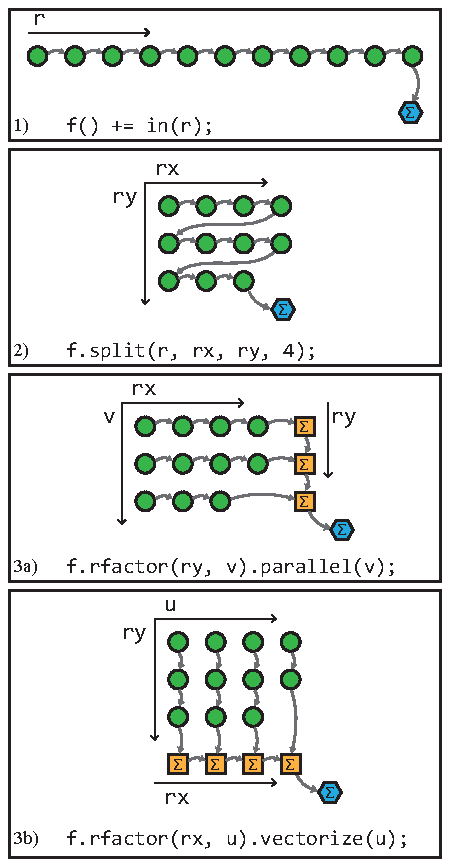
\includegraphics[width=3.2in]{rfactor}
\caption{
\code{split} followed by \code{rfactor} used to vectorize or parallelize a one-dimensional summation. 1) A serial summation of 11 elements over a one-dimensional domain \code{r}. 2) The \code{split} scheduling directive reshapes the domain into a two-dimensional reduction. The reduction is still serial. 3a) The \code{rfactor} directive creates and returns a new (orange) \emph{intermediate} stage which computes partial results along each row. The intermediate stage is now data parallel over its outer loop, which is now indexed with the new pure variable \code{v}. The merge stage (blue) retains only the serial loop over the reduction variable \code{ry}. We have \emph{reassociated} the summation. 3b) Alternatively, one can use rfactor to make the \emph{inner} loop data parallel. This can be used to vectorize reductions. The intermediate stage computes sums of whole vectors, data parallel across the vector lanes, and then the merge stage sums the lanes of the vector result. The strategy in 3a and 3b can be combined to both vectorize \emph{and} parallelize a summation.
}
\label{fig:rfactor}
\end{figure}

\code{rfactor} further separates the \emph{algorithm} from its \emph{schedule} by making it possible to factor reductions using the schedule alone. In addition to the readability and portability benefits, this means that tools that automatically generate schedules (\cite{Mullapudi:2016:ASH:2897824.2925952},\cite{Ragan-Kelley:2013:HLC:2491956.2462176}) are now capable of parallelizing reductions, which was previously a task outside of their purview.

Our work makes the following contributions:
\begin{itemize}
  \item We introduce a new Halide scheduling primitive \code{rfactor} which factors a Halide reduction into pair of reductions: an \emph{intermediate} stage that computes partial results over slices of reduction domain and \emph{merge} stage that combines those partial results;
  \item We descibe a method for automatic synthesis of an equivalent associative binary reduction operator and its identity from a serial reduction expressed as an imperative Halide \emph{update}.
  \item We implement a new stage in the Halide compiler that matches arbitrary reductions with a set of XXX fragments that are pre-generated using our synthesis method, and show that this enables the compiler to effectively transform a large set of reductions into their parallel equivalents.
\end{itemize}

The paper is structured as follows. Section~\ref{background} provides background on Halide and a discussion of related work. Section~\ref{assoc_red} presents the \code{rfactor} scheduling primitive and how it transforms Halide programs. Section~\ref{synthesize} describes the associative binary reduction operator synthesis technique. Section~\ref{evaluation} describes limitations of the technique, and demonstrates that this technique does indeed produce the expected performance gains from vectorization and parallelization.

\begin{lstlisting}[
caption = {Halide sum reduction over a one-dimensional vector.}, label={lst:sum}]
Func out;
out() = 0;
RDom r(0, input.width());
out() = out() + input(r.x);
\end{lstlisting}

\begin{lstlisting}[
caption = {Halide reduction which finds the complex number with the greatest magnitude and its location in a two-dimensional array.}, label={lst:complex_magnitude}]
Func out;
out() = {0, 0, 0, 0};
RDom r(0, input.width(), 0, input.height());
Expr real = input(r.x, r.y)[0];
Expr imag = input(r.x, r.y)[1];
Expr mag = real * real + imag * imag;
Expr best_mag = out()[0] * out()[0] +
                out()[1] * out()[1];
Expr c = mag > best_mag;
out() = {select(c, real, out()[0]),
         select(c, imag, out()[1]),
         select(c, r.x, out()[2]),
         select(c, r.y, out()[3])};
\end{lstlisting}


\section{Background and Related Work}
Programmer defines \emph{algorithm} in Halide through a Halide \emph{function}. Halide \emph{function} consists of sequence of stages, and is the unit by which we schedule things. By default, each of these stages represents a perfectly-nested loop nests in which a single value of the \emph{function} is computed and stored in the innermost loop per iteration. Stages beyond the first are called \emph{update} stages, and are allowed to recursively refer to the function. Some of the loops are data parallel and are constrained to be race-condition free by syntactic restrictions. These are represented as \code{Var}s. The bounds of these loops are inferred by Halide using interval arithmetic. Some other loops may have user-specified bounds and a user-specified nesting order, and fewer syntactic restrictions on their use. These are known as \code{RVar}s, which comprise \code{RDom}s. \code{RVar}s are used to express reductions, scattering, scans, etc. Each of these loop types, \code{Var} and \code{RVar}, can be manipulated in various ways through Halide scheduling primitives: they can be tiled, unrolled, mutually interchanged, etc., provided that the nesting order of \code{RVar}s is respected. 

While \code{Var}s are safe to parallelize or vectorize by construction -- \code{Var}s represents the naturally data-parallel axes of an \emph{algorithm} -- , \code{RVar}s can be parallelized or vectorized if and only if Halide can prove that no race condition exists. This makes parallelizing or vectorizing stages that use only \code{RVar}s difficult. For example, consider the two-dimensional convolution blur kernel shown in Listing \ref{lst:blur_loopness}, which is easily parallelizable across \code{Var} $x$ and $y$. Histogram of an image (see Listing \ref{lst:histogram_loopness}), on the other hand, is harder to parallelize since its update stage only involves \code{RVar}s. In order to parallelize a reduction like histogram, one needs to be able to factorize it into slices that have no dependencies on each other.

Although there have been several works in automatic generation of parallel associative reductions from a serial reduction, most of those works assume an explicit associative binary reduction operator, which is not applicable to Halide. Since Halide does not support reduction using a binary operator as a first-class primitive, reduction in Halide is implemented through usage of non-data-parallel \code{RVar}s. For Halide to support parallel reductions, it needs to be able to deduce an equivalent binary associative reduction operator and its identity from a serial reduction expressed as an imperative Halide \emph{update}. 

Prior work by Morita et al.~\cite{Morita:2007:AIG:1250734.1250752} introduced automatic generations of divide-and-conquer parallel programs framework based on the third homomorphism theorem and derivation of weak-right inverse. However, it requires programmer to specify the leftwards and rightwards forms of the sequential function which may not be obvious to derive. Teo et al.~\cite{Teo:1997:DEP:266670.266697} proposed a method to synthesize parallel divide-and-conquer
programs from recurrence function (which has the closest form to Halide serial reduction) through induction. They first derive two equivalent pre-parallel forms of the recurrence function by applying some generalization rules and deduce the "unknowns", the intermediate and merge reduction functions, through induction of those two pre-parallel forms. Although, it can be applied to solve some complex recurrences, such as reduction of complex multiplication, it requires long derivation and is unable to deal with argmin, which requires non-trivial re-ordering of chain of select nodes during the induction steps. 

Superoptimization~\cite{Granlund:1992:EBU:143095.143146, Massalin:1987:SLS:36206.36194} searches for the shortest or most optimized way to compute a branch-free sequence of instructions, by exhaustively searching over a space of possible programs. These rewrites can then be turned into peephole optimizations in compilers. More recent work has used stochastic search~\cite{Phothilimthana:2016:SUS:2872362.2872387, Schkufza:2013:SS:2490301.2451150} and program synthesis~\cite{Lopes:2015:PCP:2737924.2737965} to find replacements for larger sequences of instructions. Smith et al.~\cite{Smith:2016:MPS:2908080.2908102} used program synthesis to automatically generate MapReduce-style distributed programs from input-output examples. 

In this work, we find equivalent replacements of a Halide reduction through a combination of enumeration and synthesis; in addition, though our domain is more restricted, we search for larger replacements than most superoptimizers.


\begin{lstlisting}[caption={Convolution blur kernel is easily parallelizable across \code{Var} $x$ adn $y$}, label={lst:blur_loopness}]
// First stage
for y in range(input.height()):
  for x in range(input.width()):
    blur[x][y] = 0
// Update stage
parallel for y in range(input.height()):
  parallel for x in range(input.width()):
    for ry in range(kernel.height()):
      for rx in range(kernel.width()):    
        blur[x][y] = 
          blur[x][y] + 
          kernel[rx][ry]*input[x+rx-1][y+ry-1] 
\end{lstlisting}

\begin{lstlisting}[caption={Histogram of an image is hard to parallelize since its update stage does not involve \code{RVar}s}, label={lst:histogram_loopness}]
// Serial version
// First stage
for x in range(256):
  hist[x] = 0
// Update stage
for ry in range(input.height()):
  for rx in range(input.width()):
    hist[clamp(int(input[rx][ry]), 0, 255)] += 1
\end{lstlisting}


\section{Associative Reduction in Halide}
\subsection{Reductions in Halide}

Serial reductions in Halide (e.g. summation over an array, histogram, etc.) are implemented using \code{RVar}s or \code{RDom}s. An \code{RVar} is an implicit serial loop, and an \code{RDom} is an ordered list of \code{RVar}s specifying a serial loop nest. Since \code{RVar}s are not trivially parallelizable or vectorizable, a programmer must manually \emph{factor} a reduction into an \emph{intermediate} function that performs reduction over distinct slices of the domain, and a \emph{merge} function that combines those partial results.

This manual manipulation is tedious and error-prone, especially when the reduction domain is non-rectangular (see Listing \ref{lst:circular_max_1}). To further complicate matters, it is hard to infer what binary reduction operator is equivalent to a Halide update definition, and even then, many binary operators are not obviously associative (e.g. $x + y + 7xy$ is in fact associative). We will defer these issues to section \ref{synthesize}, and for now assume that given a Halide update definition we can deduce the equivalent associative binary operator and its identity. Note that we do not require the binary operators to be commutative.

\subsection{The \code{rfactor} Transformation}

To remove the burden of \emph{factoring} a reduction from the programmer, we introduce a new scheduling primitive called \code{rfactor}. This splits a reduction into pair of reductions, which we will call the \emph{intermediate} stage and the \emph{merge} stage. \code{rfactor} takes as input a list of \code{<RVar, Var>} pairs. \code{RVar}s not in the list are removed from the \emph{merge} stage and lifted to the \emph{intermediate} stage. The remaining \code{RVar}s become \code{Var}s in the \emph{intermediate} stage, which allows them to be parallelized or vectorized. See Figure \ref{fig:rfactor} for a simple example. The listings below demonstrate more complex usage.

 Note that we limit the scope of \code{rfactor} to reductions where the \emph{intermediate} and \emph{merge} stages have the same equivalent binary associative reduction operator. For instance, if the equivalent binary associative reduction operator of the \emph{intermediate} stage is \code{min(x, y)}, then that of the \emph{merge} stage must also be \code{min(x, y)}. Another restriction is that the binary associative operator must have an identity, as it is used to initialize the \emph{intermediate} stage. Not all associative binary operators have identities (e.g. $2xy$, where $x, y \in \mathds{Z}$).

\begin{lstlisting}[caption={Computing the histogram of a two-dimensional image in Halide. The RDom defines an implicit loop nest over \code{r.x} and \code{r.y}. Halide will not permit either of these loops to be parallelized, as that would introduce a race condition on the += operation.}, label={lst:histogram_rfactor_1}]
// Algorithm
Func hist;
Var i;
hist(i) = 0;
RDom r(0, input.width(), 0, input.height());
hist(input(r.x, r.y)) += 1;

// Schedule
hist.compute_root();
\end{lstlisting}

\begin{lstlisting}[caption={A manually-factored histogram. The programmer has introduced an intermediate function that computes the histogram over each row of the input. This intermediate is data-parallel over y, and so it can be parallelized. The original function \code{hist} now merely sums these partial histograms. It is data-parallel over histogram buckets, and the programmer has vectorized it.}, label={lst:histogram_rfactor_2}]
// Algorithm
Func intm;
Var i, y;
intm(i, y) = 0;
RDom rx(0, input.width());
intm(input(rx, y)) += 1;

Func hist;
hist(i) = 0;
RDom ry(0, input.height());
hist(i) += intm(i, ry);

// Schedule
intm.compute_root().update().parallel(y);
hist.compute_root().update().vectorize(i, 4);
\end{lstlisting}

\begin{lstlisting}[caption={Using \code{rfactor}, the programmer can produce the same machine code as in \ref{lst:histogram_rfactor_2}, using the simpler algorithm in \ref{lst:histogram_rfactor_1}. While the schedule is more complex, recall that it is only the five lines of algorithm that determines correctness. The programmer was able to transform the code to exploit parallelism without risking introducing a correctness bug.}, label={lst:histogram_rfactor_3}]
// Algorithm
Func hist;
Var i;
hist(i) = 0;
RDom r(0, input.width(), 0, input.height());
hist(input(r.x, r.y)) += 1;

// Schedule
Var y;
hist.compute_root()
Func intm = hist.update().rfactor(r.y, y);
intm.compute_root().update().parallel(y);
hist.update().vectorize(i, 4);
\end{lstlisting}

\begin{lstlisting}[caption={Computing the maximum over a circular domain. Reduction domains need not be rectangular. In this case we use \code{RDom::where} to restrict it to the points that lie within a circle of radius 10.}, label={lst:circular_max_1}]
// Algorithm
Func max_val;
max_val() = 0;
RDom r(0, input.width(), 0, input.height());
r.where(r.x*r.x + r.y*r.y <= 100);
max_val() = max(max_val(), input(r.x, r.y));

// Schedule
max_val.compute_root();
\end{lstlisting}

\begin{lstlisting}[caption={Manually factoring this reduction requires also manipulating the predicate associated with the RDom. The identity for \code{max} is the minimum value of the type in question.}, label={lst:circular_max_2}]
// Algorithm
Func intm;
Var y;
intm(y) = input.type().min();
RDom rx(0, input.width());
rx.where(rx*rx + y*y <= 100);
intm(y) = max(intm(y), input(rx, y));

Func max_val;
max_val() = 0;
RDom ry(0, input.height());
max_val() = max(max_val(), intm(ry));

// Schedule
intm.compute_root();
    .update().parallel(y);
max_val.compute_root();
\end{lstlisting}

\begin{lstlisting}[caption={Using \code{rfactor} in the schedule can produce the same machine code from the simpler form of the algorithm.}]
// Algorithm
Func max_val;
max_val() = 0;
RDom r(0, input.width(), 0, input.height());
r.where(r.x*r.x + r.y*r.y <= 100);
max_val() = max(max_val(), input(r.x, r.y));

// Schedule
Var y;
max_val.compute_root();
Func intm = max_val.update().rfactor(r.y, y);
intm.compute_root();
    .update().parallel(y);
\end{lstlisting}




\section{Evaluation}
\begin{table}[t]
\centering
%\setlength\tabcolsep{3.5pt} % default value: 6pt
\begin{center}
\begin{tabular}{p{1in}p{1cm}ddd}
\toprule
\multicolumn{1}{C{1.3cm}}{Benchmark} & \multicolumn{1}{C{1cm}}{Data Type} & \multicolumn{1}{C{1.2cm}}{Serial (ms)} & \multicolumn{1}{C{1.2cm}}{\code{rfactor} (ms)} & \multicolumn{1}{C{1cm}}{Speed-up} \\
% Benchmark & Serial (ms) & \code{rfactor} (ms) & Speed-up \\
\midrule \\
Maximum                 & int32 &  5.54 & 1.22 &  4.5 \\
2D histogram            & int32 & 8.80 & 1.71 &  5.1 \\
4D \code{argmin}        & int8 & 28.52 & 1.07 & 26.6 \\
Complex                 & int32 & 28.53 & 2.47 & 11.5 \\
  multiplication        &       &      &      & \\
Dot product 	        & int8 & 2.34 & 0.52 &  4.5 \\
Kitchen sink            & int32 & 30.13 & 1.91 & 15.7 \\
\bottomrule
\end{tabular}
\end{center}
\caption{Benchmark results: serial reductions vs. parallel reductions using \code{rfactor}}
\label{tab:table}
\end{table}

In this section we discuss the speed-ups one can expect by using \code{rfactor} to vectorize and parallelize serial reductions. These numbers are unsurprising -- they are equivalent to the speed-ups one can attain by manually factoring Halide reductions. We benchmark the feature using a suite of reductions of varying complexity. Some operations, like large matrix multiplication or convolution, reduce along some axes and are data parallel along others. \code{rfactor} provides little benefit in these cases, as they are already straight-forward to vectorize and parallelize, so we do not include such cases. Our benchmarks are:

\begin{itemize}
\item Maximum: The maximum integer in a list.
\item Dot product: The dot product of two vectors.
\item 4D \code{argmin}: The coordinates of the minimum value in a four-dimensional volume.
\item 2D histogram: A histogram of values present in an 8-bit image.
\item Complex multiplication: The product of a list of complex numbers.
\item Kitchen sink: An 8-tuple-element reduction that simultaneously computes the sum, product, minimum, maximum, \code{argmin}, \code{argmax}, sum-of-squares, and a count of the number of even values in a list of integers. This tests exists to demonstrate we can decompose multi-valued reductions into primitive ones.
\end{itemize}

All benchmarks run on an inputs of size $2^{24}$, which is a typical number of pixels for an input image to a Halide program. The input image data types are specified in Table~\ref{tab:table}. We run the benchmarks on 8 cores of a Xeon E5-2690. In each case we use the same Halide \emph{algorithm} code, and compare the performance attainable with \code{rfactor} to the performance attainable without it. For each benchmark, we took the minimum across 10 trials where each trial is the average of 10 iterations. We measure the execution time of the pipeline, not including the compilation time. Table~\ref{tab:table} shows the results. Without \code{rfactor}, each algorithm would require almost twice as much algorithm code to reach the same performance (see Table~\ref{tab:code_reduction}). Most importantly, \code{rfactor} provides a much less error-prone way of factoring a reduction as more of the logic is in the schedule instead of the algorithm. We also measured the increase in compile times due to the call to \code{rfactor}, and found it to be consistently under three milliseconds. The time taken to search the table for a matching operator is shown in Table~\ref{tab:search_time}. The search is fast because the table is split into subtables by the root IR node type (the largest subtable has $\thicksim 2800$ entries), and the most common operations are simple, and so they are close to the top of the tables. For a non-associative operation, \code{rfactor} must search all the way to the end of the table, and ultimately returns a compile error, which takes around 1.2 ms.

Benchmarks generally fall into two categories. Either we benefit from from vectorization \emph{and} multi-core parallelism, or we benefit from multi-core parallelism alone. Histogram, maximum, and dot-product fall into the second category. The histogram benchmark cannot be cleanly vectorized, because the bulk of the work involves scattering to data-dependent locations. The dot-product and maximum benchmarks do vectorize cleanly, but underneath Halide LLVM auto-vectorizes the reference code without \code{rfactor}, so we only see a speed-up from multi-core parallelism. We used trunk LLVM as of Sept 9, 2016 to compile the benchmarks. 4D \code{argmin}, complex multiplication, and the kitchen sink test all benefit from parallelism and vectorization. Complex multiplication, dot product, and maximum all hit the memory bandwidth limit, limiting the possible benefit from parallelism.

\textbf{TODO: the HDR+ result}

\textbf{TODO: non-Halide manually parallelized version}

Note that we did not add any patterns to the tables manually; the generated fragments were sufficient for the benchmarks, the applications in the Halide open source repository, and for the HDR+ pipeline. We could, however, manually add operators to the table if necessary in the future. An example of something that would have to be added manually is quaternion multiplication as we do not generate patterns that large during table generation.

\begin{table}[t]
\centering
%\setlength\tabcolsep{3.5pt} % default value: 6pt
\begin{center}
\begin{tabular}{p{1in}ddd}
\toprule
\multicolumn{1}{C{1.5cm}}{Benchmark} & \multicolumn{1}{C{1.3cm}}{Serial (lines)} & \multicolumn{1}{C{1.3cm}}{\code{rfactor} (lines)} & \multicolumn{1}{C{1.5cm}}{Reduction (\%)} \\
% Benchmark & Serial (ms) & \code{rfactor} (ms) & Speed-up \\
\midrule \\
Maximum                 &  9 & 5 & 44.4 \\
2D histogram            &  6 & 4 & 33.3 \\
4D \code{argmin}        &  24 & 13 & 45.8 \\
Complex                 &  12 & 7 & 41.7 \\
  multiplication        &       &       \\
Dot product 	        &  9 & 5 & 44.4 \\
Kitchen sink            & 45 & 17 & 62.2 \\
\bottomrule
\end{tabular}
\end{center}
\caption{Using \code{rfactor} reduces the lines of code in the benchmarks by 45\% on average. Only the lines of code required to define the reduction functions and \code{rfactor} calls are included in the calculation.}
\label{tab:code_reduction}
\end{table}

\begin{table}[t]
\centering
%\setlength\tabcolsep{3.5pt} % default value: 6pt
\begin{center}
\begin{tabular}{p{1in}dd}
\toprule
\multicolumn{1}{C{1.5cm}}{Benchmark} & \multicolumn{1}{C{1.5cm}}{Search time (ms)} & \multicolumn{1}{C{2cm}}{Total compilation time (ms)} \\
% Benchmark & Serial (ms) & \code{rfactor} (ms) & Speed-up \\
\midrule \\
Maximum                 &  0.08 & 127.5 \\
2D histogram            &  0.09 & 220.9 \\
4D \code{argmin}        &  0.57 & 196.2 \\
Complex                 &  0.21 & 150.4 \\
  multiplication        &       &       \\
Dot product 	        &  0.12 & 131.2 \\
Kitchen sink            &  0.55 & 187.1 \\
\bottomrule
\end{tabular}
\end{center}
\caption{The time taken to search the table to find a matching operator is relatively small with respect to the total compilation time.}
\label{tab:search_time}
\end{table}

%We ran the binary associative operator generator for 1.5 days for both the single- and two- dimensional tuples of signed 32-bit integers and unsigned 32-bit integers. We found around 10,000 associative operators in total for signed 32-bit integer single-dimensional tuple and around 6,000 for unsigned 32-bit integer single-dimensional tuple. For the two-dimensional tuple, we found around 300 operators for both signed 32-bit integer and unsigned 32-bit integer (see Table \ref{tab:int32_ops} and \ref{tab:uint32_ops}). Note that there are quite a few associative operators for the two-dimensional tuple we rejected during generation as they are decomposable into two one-dimensional associative operator.

%\begin{table*}[h!]
%\caption{Precomputed table size for single- and two- dimensional tuples of signed 32-bit integers generated in 1.5 days.}
%\label{tab:int32_ops}
%\centering
%\setlength\tabcolsep{3.5pt} % default value: 6pt
%\begin{center}
%\begin{tabular}{p{10cm}d}
%\toprule
%\multicolumn{1}{C{10cm}}{Tuple Size} & \multicolumn{1}{C{3cm}}{Size}\\
%\midrule
%Single-dimensional (with constant, no \code{select}, max of 8 leaves) & 7737 \\
%Single-dimensional (with constant, \code{select} only, max of 3 leaves for conditional, 4 leaves for the true/false) & 3162 \\
%Two-dimensional (with constant, no \code{select}, max of 7 leaves) & 327 \\
%\bottomrule
%\end{tabular}
%\end{center}
%\label{default}
%\end{table*}

%\begin{table*}[h!]
%\caption{Precomputed table size for single- and two- dimensional tuples of unsigned 32-bit integers generated in 1.5 days.}
%\label{tab:uint32_ops}
%\centering
%\setlength\tabcolsep{3.5pt} % default value: 6pt
%\begin{center}
%\begin{tabular}{p{10cm}d}
%\toprule
%\multicolumn{1}{C{10cm}}{Tuple Size} & \multicolumn{1}{C{3cm}}{Size}\\
%\midrule
%Single-dimensional (with constant, no \code{select}, max of 8 leaves) & 5813 \\
%Single-dimensional (with constant, \code{select} only, max of 3 leaves for conditional, 4 leaves for the true/false) & 518 \\
%Two-dimensional (with constant, no \code{select}, max of 7 leaves) & 348 \\
%\bottomrule
%\end{tabular}
%\end{center}
%\label{default}
%\end{table*}

%Discussion

%Synthetic functions (also to show limitations): approximating 128-bit add with 2 64-bit integers -> z3 cannot prove that it is associative, although the max/min forms are provable with z3. \\

%Limitations: we need an identity, symmetric intermediate and merge functions: they should be of the same form, constrained by the look-up table (we can only match to whatever are in the table -> whatever z3 can prove to be associative) + whatever we thought to generate. Some associative ops (e.g. 4x4 matrix multiply) are just expensive to generate. Technically it's doable, provided we limit the ops to addition and multiplication and restricting the variables involved in the expr to be unique (no repeats) during lookup table generation. Other ops may not be covered in our search (e.g. one that exploits a special property unique to some large constant). \\

%Real-world stuff: same code that can be simplified (reducing number of lines of code, etc) when using rfactor \\

%Performance of generation/search/synthesis. <TODO: Not sure what this is about? time taken when doing the matching? how many associative operations can be generated within some hours? > \\

%Case study of importance of "code reduction"? <TODO: Not sure what this is about? SK: I think the idea is that without the approach in this paper, you have to write more code (= more bugs) but also that you have to write arch-specific code (if you want to do parallel reduction on one arch and not the other) > \\


\section{Discussion}
(Don't forget to reiterate limitations)


\bibliographystyle{abbrv}
\bibliography{sigproc}  % sigproc.bib is the name of the Bibliography in this case
% You must have a proper ".bib" file
%  and remember to run:
% latex bibtex latex latex
% to resolve all references
%
% ACM needs 'a single self-contained file'!
%
\end{document}
